\documentclass[../main.tex]{subfiles}
\graphicspath{{\subfix{..}}}

\begin{document}
\chapter{Reliability of machine learning methods}
\label{sec:janne}

\epigraph{``Psychohistory was the quintessence of sociology; it was the science of human behavior reduced to mathematical equations. The individual human being is unpredictable, but the reactions of human mobs, Seldon found, could be treated statistically''}{Isaac Asimov, Second Foundation}

\minitoc

As explained in previous chapters, JUNO is a precision experiment where the complete understanding of the effects at hand is crucial. As it will be illustrated in Chapter \ref{sec:joint_fit}, even small invisible biases or uncertainties could lead to the imposibility to run the measurements, or even worse, wrong our mass ordering measurements. While the liquid scintillator technology is well none and straightforward, this is the first time it is deployed to such scale, and for such precision. This novelty bring its fair share of elements, effects or assumption, that, if they were to be overlooked, could cause issue.

We already shown a large variety of reconstruction algorithms, OMILREC for LPMT reconstruction in section \ref{sec:juno:reco}, numerous machine learning algorithms in section \ref{sec:juno:ml} and our own work in chapters \ref{sec:jcnn} and \ref{sec:jgnn}. Those algorithms were compared to each others based on their performance as in \cite{qian_vertex_2021} but we are the first that looked into the correlation between the reconstruction. The combinations of algorithms shown in Chapter \ref{sec:jcnn} and Chapter \ref{sec:jgnn} show that some information elude the algorithms. We used this fact to try to improve our performance but this could also lead the algorithm to being vulnerable to some effect that could affect the detector and wrong the measurements.

The search for such effect could be done by hand, but the process would be tedious. We propose in this thesis a machine learning method to probe for those effects.  In section \ref{sec:janne:method}, I describe the method behind the algorithm. In section \ref{sec:janne:arch} I detail the architecture of our algorithm and in section \ref{sec:janne:results} the results of it. Finally, in section \ref{sec:janne:conclusion}, I conclude and discuss about the prospect and possible improvements to bring to this work.

\section{Method}
\label{sec:janne:method}
%\begin{itemize}
%  \item JUNO needs very good understanding of reconstruction
%  \item Estimator combination shows that there can be improvement due to simplfication and that NN/reco methods can have hard time grasping all the detector effect.
%  \item If there is potential failure point, we need to search for them
%  \item La mesure de la NMO est tres sensible (see $alpha_{qnl}$ joint fit chapter)
%\end{itemize}

As introduced above, JUNO needs a very good understanding of the biases and effects affecting its reconstruction as a small bias could wrong the mass ordering measurement. To calibrate those biases and effect, JUNO rely on multiples sources that can be located at various point in the detector. The calibration strategy was already discussed in section \ref{sec:juno:calib} and show calibrations sources of gammas, neutrons and positrons, with the catch that the positrons will annihilate inside the encapsulation and only the two 511 keV gammas will be seen.

None of the calibrations sources considered are positron event. While electrons and positrons events should be pretty similar in their interaction with the electronic cloud of the LS atoms, electron events are missing the two annihilations $\gamma$ and the potential of forming a positronium \cite{schwarz_measurements_2018}. The topology of the event thus differ of the order of magnitude of our reconstruction performance: a few nanoseconds for the energy deposit and positronium annihilation against a time transit spread between 3 and 6 ns depending on the PMT type \cite{rodphai_20-inch_2021, liao_study_2017, li_characterization_2018} and the $\gamma$ will travel distances of the order of magnitude of the typical LPMT resolution of 8 cm (see section \ref{sec:juno:reco}).

Another natural calibration source is the $^{12}B$ spectrum. The $^{12}B$ is a cosmogenically produced isotope through the passage of muons inside the LS. The $^{12}B$ decays via $\beta^-$ emissions with a Q value of 13.5 MeV with more than 98\% of the decay resulting in ground state $^{12}C$. The $^{12}B$ event will be cleanly identified by looking for delayed high energy $\beta$ events after an energetic muon. Due to its natural causes, the $^{12}B$ events will be uniformly distributed in the detector. The calibration strategy consist in fitting the energy spectrum of $^{12}B$ with the results of the simulation to adjust the simulation parameters. Both sources will be used to \textit{control} the response of the detector.

Unlike lasers and radioactive, from which the localization and energy will be well known, the individual truth of $^{12}B$ will be unknown with only the localisation loosely constrained by the muon track. Only higher order observables such as the energy distribution will be accessible.

All of those considerations could hide potential unknown or undetected effect that could lead to issue in the mass ordering analysis. But, while we have idea from where the issue could come, the production by hand of event perturbations that go unseen in the calibration would be tedious. That's why we propose to use a Neural Network to produce those perturbations if they exists. A schematic of the concept is presented in figure \ref{fig:janne:method:schema}.

\begin{figure}[ht]
  \centering
  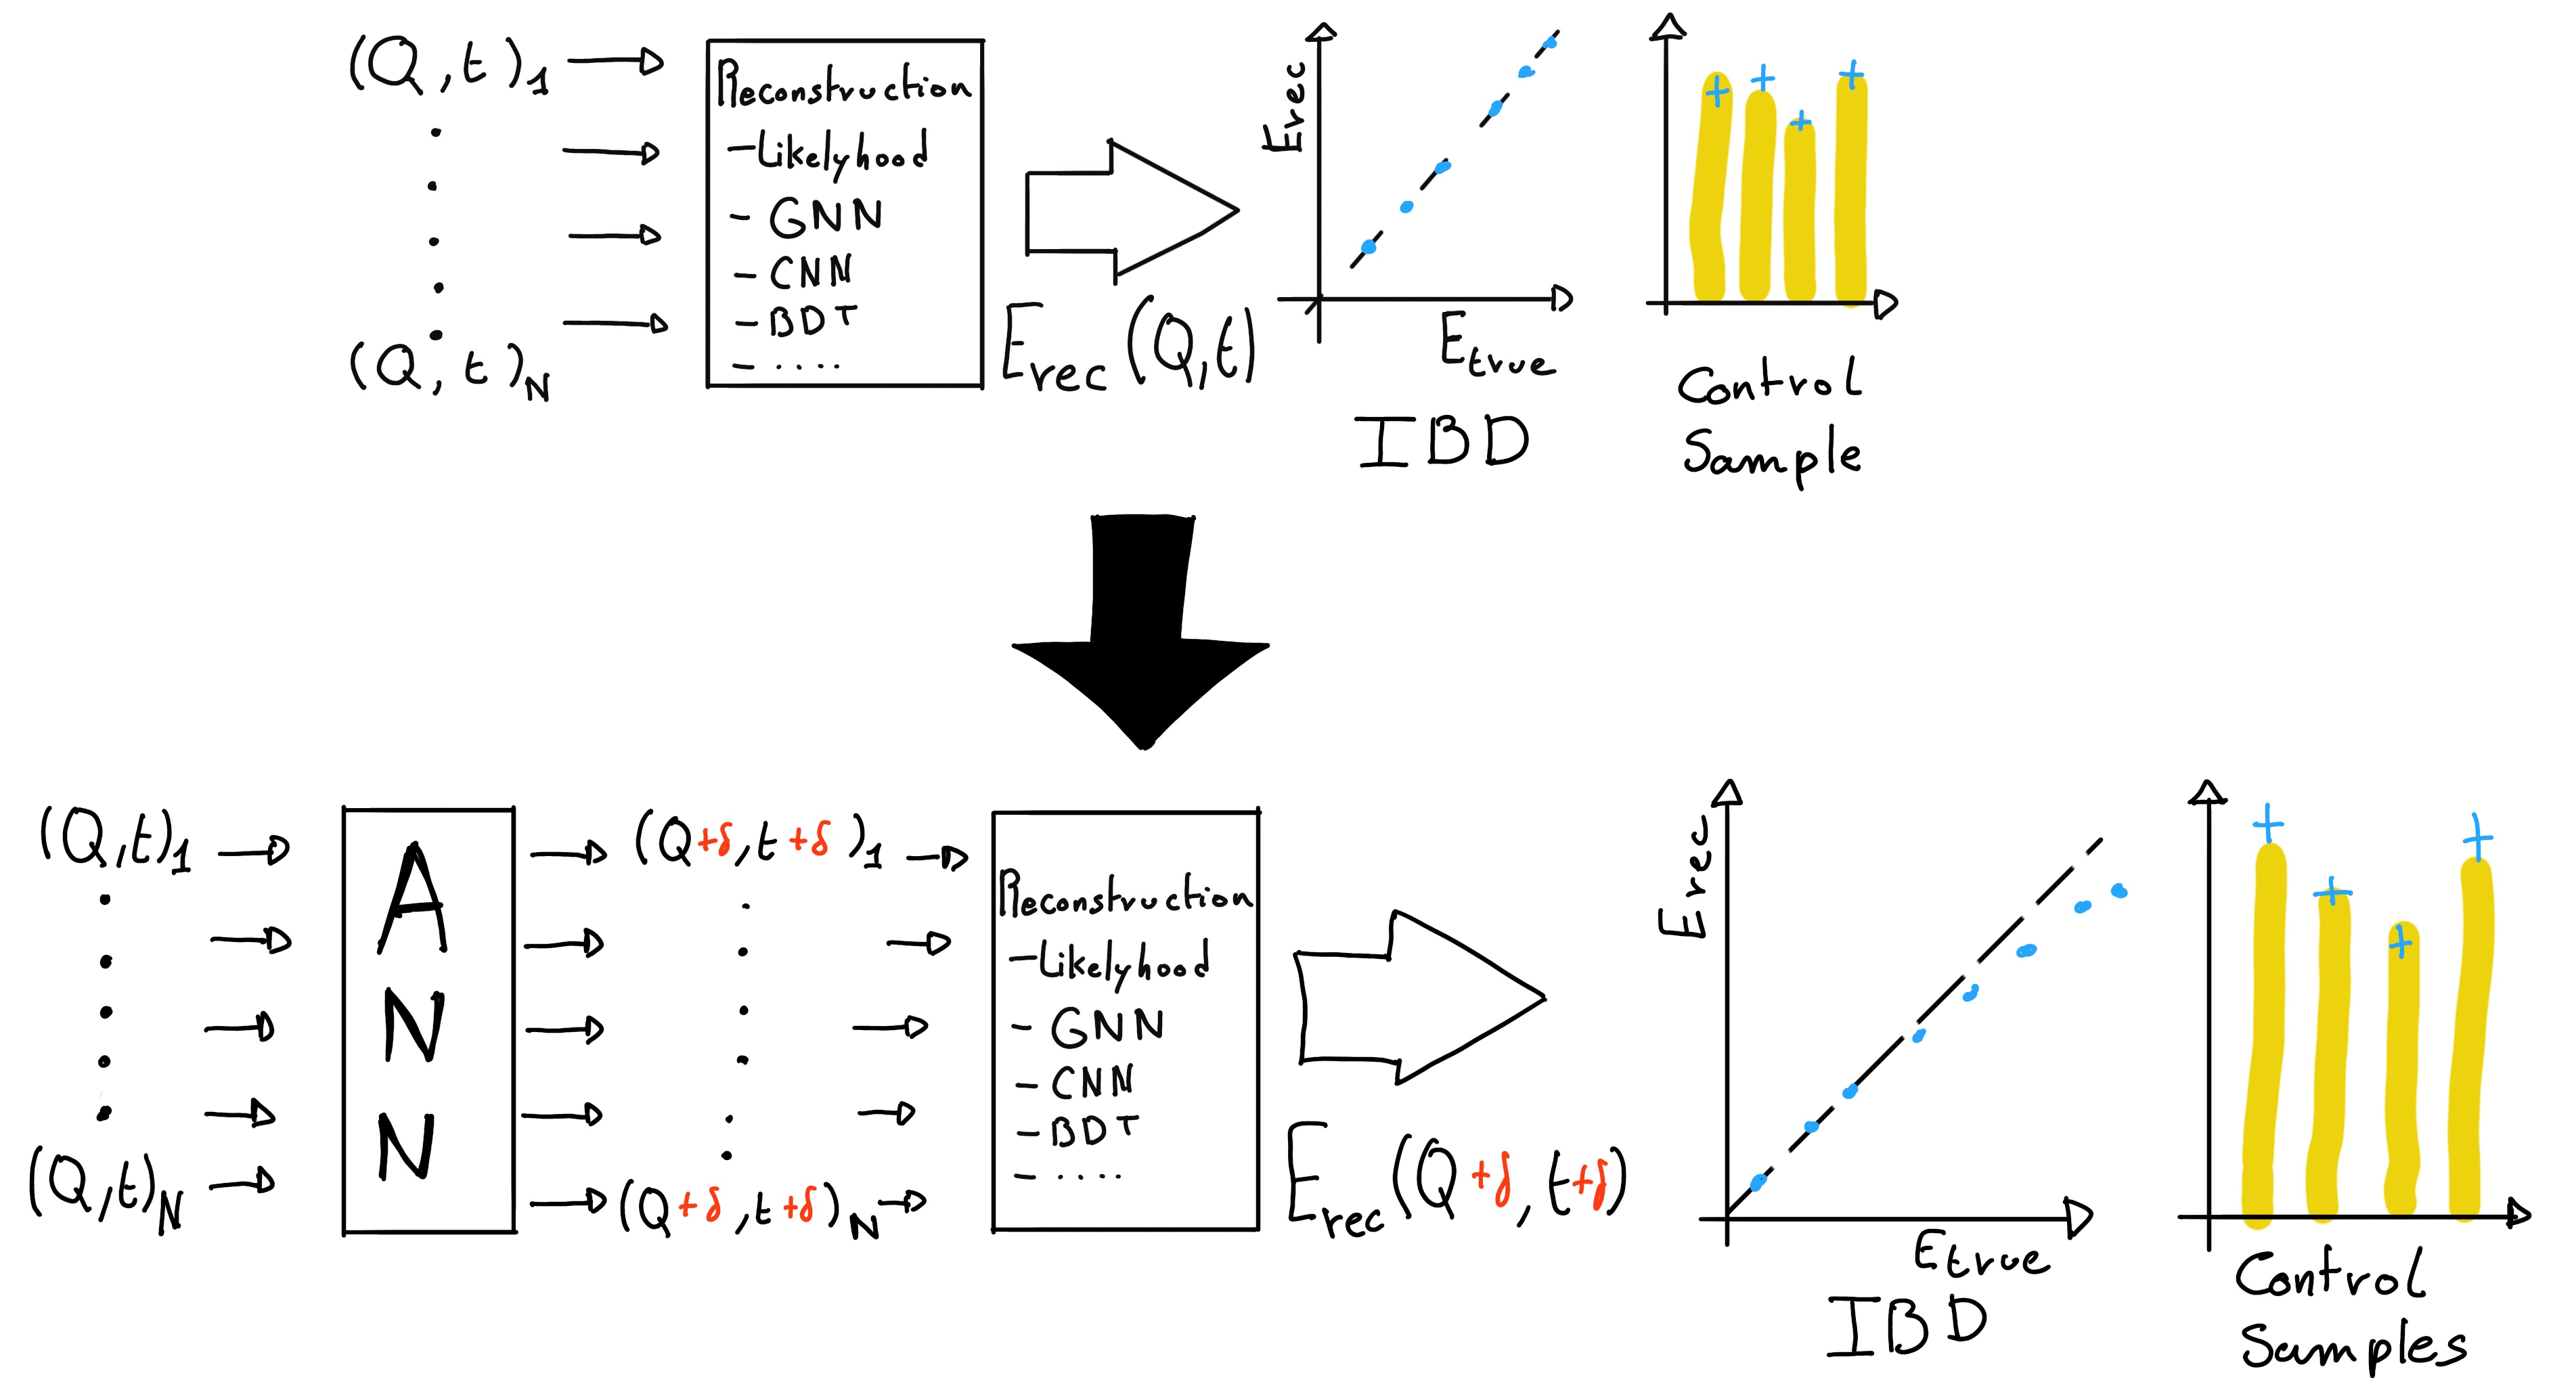
\includegraphics[width=\linewidth]{images/janne/ann_method.jpg}
  \caption{Schema of the method to discover vulnerabilities in the reconstruction methods. \textbf{On the top} of the image, the standard data flow. The individual charge and times are fed to a reconstruction algorithm. From the reconstructed energies, we can produce an IBD spectrum and compute control observables from the control samples. \textbf{On the bottom}, the same data flow but we add an ANN between the input and the reconstruction. The ANN will slightly change the input charge and time so the reconstruction algorithm inaccurately reconstruct the IBD energy, but the perturbation is not visible in the control sample.}
  \label{fig:janne:method:schema}
\end{figure}

This network should produce physically sound perturbation, that would not be seen by the calibration but also by the visualisation of the event. If the ANN manage to produce such perturbations, we can derive systemic uncertainties from it. If it fail to find some, it is a proof of robustness for the attacked reconstruction method.

For this study we consider a ``physics'' dataset composed of 1M positron events from J23, uniformly distributed in the Central Detector (CD) and in deposited energy between $E_{dep} \in [1.022; 10.022]$. This set represent the IBD events we want to \textit{wrongly} reconstruct.

We use a second ``control'' dataset of electron event also uniformly distributed in the detector and over the same energy range. They mimic the energy deposit of $^{12}B$ decay and are used as the sample to compute the control observables.

\section{Architecture}
\label{sec:janne:arch}
%\begin{itemize}
%  \item Expliquer la problematique dans l'architecture
%  \item Ambition de pouvoir etre appliqué a toutes les methodes, pas que NN
%  \item Pb techique: descente de gradient
%  \item Présenter la loss
%\end{itemize}
We can describe the goal of the ANN by the following loss function:
\begin{equation}
  \label{eq:janne:loss}
  \mathcal{L} = \mathcal{L}_{adv} + \mathcal{L}_{reg}
\end{equation}
where $\mathcal{L}_{adv}$ is the adversarial loss, which is minimum when the reconstruction is completely broken. We thus need to define what is a \textit{wrong} reconstruction. We choose to define it via the correlation between the reconstructed and deposited energy
\begin{equation}
  \mathcal{L}_{adv} = |\mathrm{Corr}(E_{rec}, E_{dep})|
\end{equation}
which is positive or null and is minimal when the reconstructed energy is decorrelated with the deposited energy, the reconstruction is wrong.

The term $\mathcal{L}_{reg}$ is the regularisation term, which is minimal when the control variable are correctly reconstructed
\begin{equation}
  \mathcal{L}_{reg} = \sum_\lambda (O^{rec}_\lambda - O^{th}_\lambda)^2
\end{equation}
where $\lambda$ index the different control observables that will be considered in this study. It's minimal when the control observables after perturbation $O^{rec}_\lambda$ are coherent with their expected values $O^{th}_\lambda$.

We see that the final loss is the equilibrium between the adversarial and regularisation loss.

\subsection{Back-propagation problematic}

We would like this method to be applicable to any kind of reconstruction algorithm but this complicated considering standard training method through backward-propagation, discussed in details in section \ref{sec:ml:optim}. For explanation, let's define the application of the reconstruction algorithm as $\mathcal{F}$ on an event $X$, resulting in the prediction $Y$ and the application of the ANN $\mathcal{G}$ on $X$ to give a perturbed event $X'$, we can parametrize the equation \ref{eq:janne:loss}
\begin{align}
  Y = \mathcal{F}(X); ~~& Y' = \mathcal{F}(X') = \mathcal{F}(\mathcal{G}(X))
\end{align}
\begin{equation}
  \mathcal{L} \equiv \mathcal{L}(\mathcal{F}(\mathcal{G}(X)), Y_t)
\end{equation}
where $Y_t$ is the reconstruction target of $Y$.

Now if we consider a parameter $\bm{\theta}$ of the ANN on which we want to optimize $\mathcal{L}$, in the backward-propagation optimisation framework we need to compute
\begin{equation}
  \frac{\partial \mathcal{L}(\mathcal{F}(\mathcal{G}(X)))}{\partial \bm{\theta}}
\end{equation}
which, when using the chain rule, become
\begin{equation}
  \frac{\partial \mathcal{L}(\mathcal{F}(\mathcal{G}(X)))}{\partial \bm{\theta}} = \frac{\partial \mathcal{G}}{\partial \bm{\theta}} \cdot \frac{\partial \mathcal{F}}{\partial \mathcal{G}} \cdot \frac{\partial \mathcal{L}}{\partial \mathcal{F}}
\end{equation}

The terms $\frac{\partial \mathcal{G}}{\partial \bm{\theta}}$ and $\frac{\partial \mathcal{L}}{\partial \mathcal{F}}$ are easily computable but $\frac{\partial \mathcal{F}}{\partial \mathcal{G}}$ depends on the nature of the reconstruction algorithm. While it comes naturally when using NN algorithms, it's not so trivial for other kind of algorithms like likelihood. Solutions exists to optimize networks that work in complex, non differentiable environments, such as \textit{Deep Reinforcement Learning} \cite{kiran_deep_2021, vinyals_grandmaster_2019} but as a first prototype we will restrict ourselves to neural networks for the reconstruction algorithm.

The backward-propagation introduce a second issue. At the beginning of the subsection we introduce $X' = \mathcal{G}(X)$, the event after perturbation. It's an input of the reconstruction $\mathcal{F}$, thus, let's say that the event, in its form $X$, is a list of tuples $(id, Q, t)$ which are the hit on the PMT $id$. If $\mathcal{F}$ require the information to be formatted in a specific way (graph, images, ...) via an algorithm $\tau(X)$, it means that
\begin{equation}
  \frac{\partial \mathcal{L}(\mathcal{F}(\tau(\mathcal{G}(X))))}{\partial \bm{\theta}} = \frac{\partial \mathcal{G}}{\partial \bm{\theta}} \cdot \frac{\partial \tau}{\partial \mathcal{G}} \cdot \frac{\partial \mathcal{F}}{\partial \tau} \cdot \frac{\partial \mathcal{L}}{\partial \mathcal{F}}
\end{equation}
which also requires that $\frac{\partial \tau}{\partial \mathcal{G}}$ is differentiable.

On the other hand, if $X$ is already formatted as the input of $\mathcal{F}$, it mean that $\mathcal{G}$ take the same format as input and we drop the requirement on $\tau$ to be differentiable. Concretely, if $\mathcal{F}$ takes an image as input, it mean that $\mathcal{G}$ will also takes an image as input and output an image. That also unfortunately mean that if some informations is loss before $\mathcal{G}$, for example during the charge and time aggregation in pixels, it cannot retrieve and modify it.

A more elegant solution would that $\mathcal{G}$ would also compute the transformation $\tau$ in addition to finding relevant perturbation, but for the simplicity of this exploratory work, we use a $\mathcal{G}$ that process transformed data.

\subsection{Reconstruction Network}
\label{sec:janne:arch:reco}
%\begin{itemize}
%  \item Reseau de Neurone Simple. Deux avantages:
%  \item Besoin pour la descente de gradient
%  \item Un reseau "simpliste" a plus de chance de présenter des "défauts" que l'ANN pourrait exploiter
%\end{itemize}

As introduced just before, w need a NN algorithm for IBD reconstruction. We could have used the GNN exposed in Chapter \ref{sec:jgnn}

\subsection{Adversarial Neural Network}
\label{sec:janne:arch:ann}
\begin{itemize}
  \item Decrire l'architecture de l'ANN
\end{itemize}

\subsection{Training}
\label{sec:janne:arch:training}
\begin{itemize}
  \item Presentation du dataset
  \item 2 etapes d'entrainement
  \item Retour à l'identitié -> que l'ANN ne fasse pas n'importe quoi
  \item Cassage de la reconstruction
\end{itemize}

\subsubsection{Hyperparameter optimization}
\label{sec:janne:arch:hyper}
\begin{itemize}
  \item Pour les meme raison que l'ANN:
    \begin{itemize}
      \item Phase exploratoire, architecture tres changeante, random search n'est pas viable
      \item Architecture consomme beaucoup, besoin d'entrainer sur l'A100
      \item Possiblement que de l'optimization permetterais de faire passer sur V100, mais developement techniques necessaires.
    \end{itemize}
\end{itemize}

\section{Results}
\label{sec:janne:results}

\begin{itemize}
  \item Voir slide Gilles
\end{itemize}

\subsection{Back to identity}
\label{sec:janne:results:identity}

\subsection{Breaking of the reconstruction}
\label{sec:janne:results:break}

\section{Conclusion and prospect}
\label{sec:janne:conclusion}
\begin{itemize}
  \item Not enough
  \item Probably guide the ANN
\end{itemize}
\end{document}
